% Provenance (never printed): old premiere S / seconde material on minerals and
% rocks (identifying minerals in hand specimen, the silicates, the minerals of
% granite, basalt and peridotite, thin sections in polarised light).
% Element fractions and rock densities from figdata/grade-11/mineral_density.py
% (Rudnick and Gao 2014 bulk crust; webmineral mean densities). Mineral, crystal,
% rock families and the Mohs scale are Book 1's (grade 6): recalled, not defined.
% Felsic and mafic belong to g11.08: not used here.
\chapter{Os minerais}\label{ch:g11:minerals}

Pegue um seixo de granito e olhe para ele com uma lupa. Ele não é uma única
substância, mas um mosaico de grãos encaixados uns nos outros: grãos
cinzentos, vítreos e quase transparentes; grãos cor-de-rosa, em blocos,
cujas faces quebradas brilham à luz quando se gira o seixo; pequenas
lamelas pretas que a ponta de uma faca levanta em folhas finas. Cada tipo de
grão é um mineral. Este capítulo mostra como um geólogo os distingue, por
que quase todos são construídos de silício e oxigênio, como eles formam as
rochas vistas até aqui --- granito, basalto, \omterm{def:g11:ocean-ridges:peridotite}{peridotito} --- e como uma fatia
de rocha mais fina que um fio de cabelo, vista em luz polarizada, mostra
todos eles de uma vez.

\begin{omfigure}
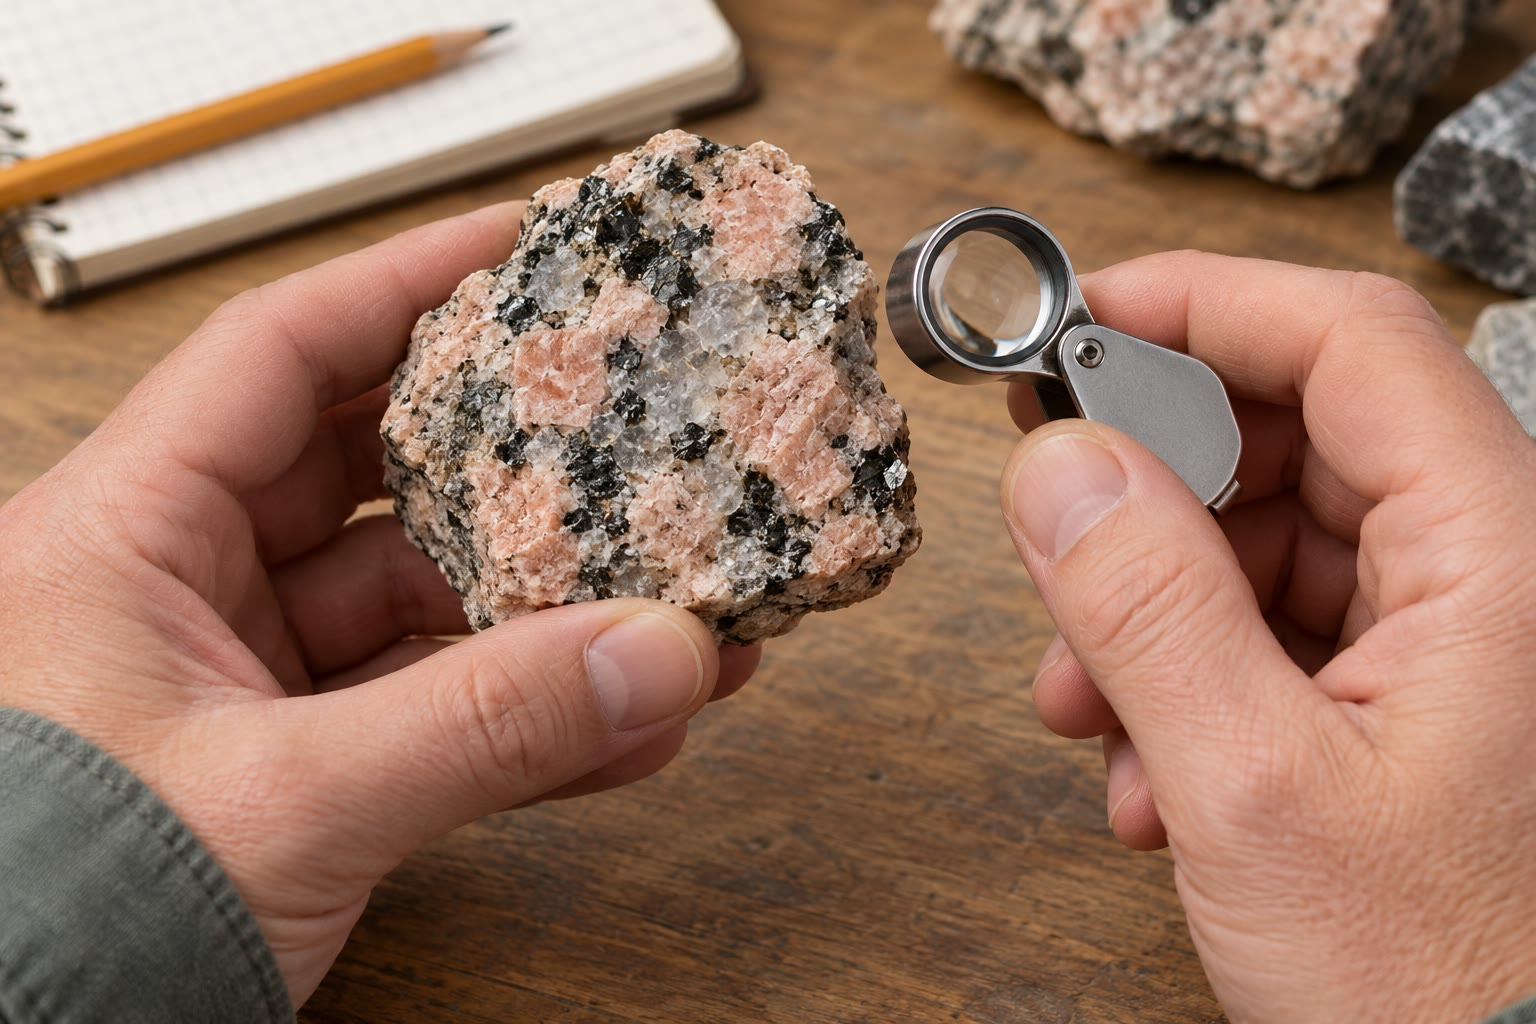
\includegraphics[width=0.62\linewidth]{images/book2/ai/g11-geologist-hand-lens.jpg}

{\small Um granito examinado com uma lupa: a primeira ferramenta para
distinguir os minerais. (Ilustração gerada por IA.)}
\end{omfigure}

\begin{recall}
Um mineral é uma substância sólida natural, não produzida por seres vivos,
de composição fixa e com os átomos arranjados de modo regular; uma rocha é
feita de um ou de vários minerais. O granito é feito principalmente de
feldspato, quartzo e mica. As rochas se dividem em três famílias: ígneas,
sedimentares e metamórficas. A dureza de um mineral é a sua resistência a
ser riscado, classificada de 1 (talco) a 10 (diamante) na escala de Mohs; o
feldspato ortoclásio tem 6 e o quartzo 7, enquanto uma placa de vidro tem
cerca de 5.5 e um prego de aço cerca de 6.5 (Livro 1, 6º ano). A densidade
de um corpo é a sua massa dividida pelo seu volume (física). Um composto é
descrito por uma fórmula que conta os seus átomos; num sólido feito de íons,
as cargas positivas e negativas se equilibram (química). O \omterm{def:g11:ocean-ridges:peridotite}{peridotito} forma
o manto; o \omterm{def:g11:ocean-ridges:gabbro}{gabro} e o basalto formam a \omterm{def:g11:ocean-ridges:oceanic-lithosphere}{crosta oceânica}
(\cref{ch:g11:ocean-ridges}).
\end{recall}
% ledger: usgs:mineral-rock, nps:granite-minerals, nps:mohs-ladder, nps:mohs-testers

\section{Distinguir os minerais}

Um mineral tem uma composição fixa e um arranjo regular de átomos. As duas
coisas aparecem por fora: na forma dos seus cristais, no modo como ele se
quebra, no modo como reflete a luz, na sua dureza e na sua densidade.
Nenhuma dessas propriedades basta sozinha; juntas, elas identificam os
minerais comuns numa amostra de mão, sem outro instrumento além de uma lupa,
um prego de aço e uma placa de vidro.

\paragraph{A forma.} Um cristal que cresceu livremente, numa cavidade ou num
líquido, assume uma forma que reflete o arranjo dos seus átomos.

\begin{definition}[Hábito]\label{def:g11:minerals:habit}
O \emph{hábito}\index{habito (de um cristal)@hábito (de um cristal)} de um
mineral é a forma geral que os seus cristais assumem: cúbico, tabular (plano,
como uma placa), prismático (alongado, como um prisma), laminar, acicular
(em forma de agulha), e assim por diante.
\end{definition}
% ledger: tulane:physprop

O quartzo cresce em prismas de seis faces terminados em pontas; a biotita,
em placas planas de seis lados (fotografias abaixo). Na maioria das rochas,
porém, os grãos cresceram uns contra os outros e não têm faces próprias: o
\omterm{def:g11:minerals:habit}{hábito} então diz pouco, e as outras propriedades assumem o papel.
% ledger: photo:g11-quartz, photo:g11-biotite

\paragraph{A cor e o brilho.} A cor é a primeira coisa que se vê, e a menos
confiável. Um traço de outro elemento basta para mudá-la: o quartzo pode ser
incolor, branco, preto, rosa, azul ou roxo. Alguns minerais, por outro lado,
quase não variam: a olivina é quase sempre verde. O modo como um mineral
reflete a luz é um guia melhor.
% ledger: tulane:physprop

\begin{definition}[Brilho]\label{def:g11:minerals:lustre}
O \emph{brilho}\index{brilho} de um mineral é o seu aspecto à luz refletida.
Ele é \emph{metálico} quando o mineral brilha como um metal, e não metálico
nos outros casos: \emph{vítreo} (como vidro, como o quartzo), nacarado,
resinoso, e assim por diante.
\end{definition}
% ledger: tulane:physprop

\paragraph{O modo como se quebra.} Golpeie um cristal e ele se quebra. Onde
as ligações entre os seus átomos são mais fracas ao longo de certos planos,
ele se parte ao longo deles, várias e várias vezes, em superfícies planas e
brilhantes; onde nenhum plano é mais fraco que outro, ele se quebra ao longo
de qualquer superfície.

\begin{definition}[Clivagem; fratura]\label{def:g11:minerals:cleavage}
A \emph{clivagem}\index{clivagem (de um mineral)} é a tendência de um mineral
a se partir ao longo de planos, paralelos a direções em que as ligações
entre os seus átomos são mais fracas. A \emph{fratura}\index{fratura (de um mineral)}
é a ruptura ao longo de superfícies irregulares, num mineral sem plano de
fraqueza; uma fratura de superfícies lisas e curvas, como as de um vidro
quebrado, é chamada \emph{conchoidal}.
\end{definition}
% ledger: tulane:physprop

Um mineral pode ter uma \omterm{def:g11:minerals:cleavage}{clivagem}, duas, três ou nenhuma. As micas têm uma,
perfeita: elas se desfolham em lâminas. Os feldspatos têm duas. O quartzo
não tem nenhuma: ele se quebra com uma \omterm{def:g11:minerals:cleavage}{fratura} conchoidal, o que o distingue
de imediato de um feldspato da mesma cor cinza ou branca. O ângulo entre
duas clivagens é fixado pelo arranjo dos átomos, e pode ser medido num grão
quebrado ou num corte: as duas clivagens de um piroxênio se encontram a
cerca de \ang{87} e \ang{93}, quase em ângulo reto; as de um anfibólio a
cerca de \ang{56} e \ang{124}. Os piroxênios e os anfibólios são muitas
vezes escuros e parecidos; os seus ângulos de \omterm{def:g11:minerals:cleavage}{clivagem} os distinguem.
% ledger: wm:densities (quartz conchoidal; orthoclase two cleavages; biotite one), tulane:cleavage-angles

\begin{omfigure}
\begin{tikzpicture}[font=\footnotesize]
  % pyroxene: octagonal cross-section, cleavage traces at 46.5 and 133.5 degrees (87/93)
  \begin{scope}
    \coordinate (p1) at (1,0.4); \coordinate (p2) at (0.431,1); \coordinate (p3) at (-0.431,1);
    \coordinate (p4) at (-1,0.4); \coordinate (p5) at (-1,-0.4); \coordinate (p6) at (-0.431,-1);
    \coordinate (p7) at (0.431,-1); \coordinate (p8) at (1,-0.4);
    \begin{scope}[scale=1.5]
      \fill[black!72!green!40] (1,0.4) -- (0.431,1) -- (-0.431,1) -- (-1,0.4) -- (-1,-0.4) -- (-0.431,-1) -- (0.431,-1) -- (1,-0.4) -- cycle;
      \clip (1,0.4) -- (0.431,1) -- (-0.431,1) -- (-1,0.4) -- (-1,-0.4) -- (-0.431,-1) -- (0.431,-1) -- (1,-0.4) -- cycle;
      \foreach \s in {-5,...,5} {
        \draw[white!85!black, line width=0.5pt] ($(136.5:\s*0.24)+(46.5:-3)$) -- ($(136.5:\s*0.24)+(46.5:3)$);
        \draw[white!85!black, line width=0.5pt] ($(223.5:\s*0.24)+(133.5:-3)$) -- ($(223.5:\s*0.24)+(133.5:3)$);}
      \draw[black!80, line width=0.9pt] (46.5:-3) -- (46.5:3); \draw[black!80, line width=0.9pt] (133.5:-3) -- (133.5:3);
    \end{scope}
    \draw[black!70, line width=0.7pt, scale=1.5] (1,0.4) -- (0.431,1) -- (-0.431,1) -- (-1,0.4) -- (-1,-0.4) -- (-0.431,-1) -- (0.431,-1) -- (1,-0.4) -- cycle;
    \draw[omProp, line width=1pt] (46.5:0.75) arc[start angle=46.5, end angle=133.5, radius=0.75];
    \draw[omDef, line width=1pt] (133.5:0.5) arc[start angle=133.5, end angle=226.5, radius=0.5];
    \node[fill=white, inner sep=1pt, text=omProp!80!black] at (90:0.98) {\ang{87}};
    \node[fill=white, inner sep=1pt, text=omDef] at (180:0.82) {\ang{93}};
    \node[anchor=north, align=center] at (0,-1.7) {\strut\textbf{piroxênio}\\clivagens a cerca de \ang{87} e \ang{93}};
  \end{scope}
  % amphibole: elongated hexagon, cleavage traces at 28 and 152 degrees (56/124 opening sideways)
  \begin{scope}[xshift=6.2cm]
    \begin{scope}[scale=1.5]
      \fill[black!72!green!40] (1.6,0) -- (0.62,0.52) -- (-0.62,0.52) -- (-1.6,0) -- (-0.62,-0.52) -- (0.62,-0.52) -- cycle;
      \clip (1.6,0) -- (0.62,0.52) -- (-0.62,0.52) -- (-1.6,0) -- (-0.62,-0.52) -- (0.62,-0.52) -- cycle;
      \foreach \s in {-6,...,6} {
        \draw[white!85!black, line width=0.5pt] ($(118:\s*0.2)+(28:-4)$) -- ($(118:\s*0.2)+(28:4)$);
        \draw[white!85!black, line width=0.5pt] ($(242:\s*0.2)+(152:-4)$) -- ($(242:\s*0.2)+(152:4)$);}
      \draw[black!80, line width=0.9pt] (28:-4) -- (28:4); \draw[black!80, line width=0.9pt] (152:-4) -- (152:4);
    \end{scope}
    \draw[black!70, line width=0.7pt, scale=1.5] (1.6,0) -- (0.62,0.52) -- (-0.62,0.52) -- (-1.6,0) -- (-0.62,-0.52) -- (0.62,-0.52) -- cycle;
    \draw[omProp, line width=1pt] (-28:0.75) arc[start angle=-28, end angle=28, radius=0.75];
    \draw[omDef, line width=1pt] (28:0.42) arc[start angle=28, end angle=152, radius=0.42];
    \node[fill=white, inner sep=1pt, text=omProp!80!black] at (0:1.02) {\ang{56}};
    \node[fill=white, inner sep=1pt, text=omDef] at (90:0.6) {\ang{124}};
    \node[anchor=north, align=center] at (0,-1.7) {\strut\textbf{anfibólio}\\clivagens a cerca de \ang{56} e \ang{124}};
  \end{scope}
\end{tikzpicture}

{\small Cortes de um cristal de piroxênio (à esquerda) e de um cristal de
anfibólio (à direita), feitos transversalmente ao seu comprimento (um
desenho). As linhas finas são os traços das duas clivagens, duas delas
traçadas mais grossas onde os ângulos são lidos; os ângulos entre elas,
quase retos no piroxênio, muito mais abertos e muito mais fechados no anfibólio, distinguem dois
minerais escuros que de resto são parecidos.}
\end{omfigure}
% ledger: tulane:cleavage-angles

\paragraph{A dureza e a densidade.} A dureza, vista no Livro 1, separa
minerais que se parecem: o quartzo (7) risca o vidro e não é riscado por um
prego de aço; um feldspato (6) também risca o vidro, mas o prego o risca. A
densidade é a última pista. Na mão, não se pesa um grão, mas pode-se pesar
uma amostra de um único mineral, e os minerais comuns das rochas cobrem uma
faixa estreita, de cerca de \qty{2.6}{g/cm^3} a cerca de \qty{3.4}{g/cm^3}
(gráfico abaixo): os mais leves são ricos em silício, alumínio, sódio e
potássio, os mais densos em ferro e magnésio.
% ledger: nps:mohs-ladder, nps:mohs-testers, wm:densities

\begin{method}[Identificar um mineral numa amostra de mão]\label{met:g11:minerals:identify}
\begin{enumerate}
  \item Observe a forma do grão ou do cristal (\omterm{def:g11:minerals:habit}{hábito}), a sua cor --- apenas
        como indício --- e o seu \omterm{def:g11:minerals:lustre}{brilho}.
  \item Procure a \omterm{def:g11:minerals:cleavage}{clivagem}: superfícies planas e brilhantes que refletem a
        luz juntas quando se gira a amostra. Conte as direções de \omterm{def:g11:minerals:cleavage}{clivagem} e
        estime o ângulo entre elas; se não houver nenhuma, descreva a
        \omterm{def:g11:minerals:cleavage}{fratura}.
  \item Teste a dureza com objetos de referência: uma placa de vidro (cerca
        de 5.5) e um prego de aço (cerca de 6.5).
  \item Se a amostra for de um único mineral, compare a sua densidade com as
        densidades dos candidatos.
  \item Conclua pela combinação das propriedades, nunca por uma só.
\end{enumerate}
\end{method}
% ledger: nps:mohs-testers

\begin{example}[Quartzo ou feldspato?]
Dois grãos branco-acinzentados num granito. O primeiro não mostra nenhuma
face plana, só quebras lisas e curvas, e o prego de aço não deixa marca
nele: \omterm{def:g11:minerals:cleavage}{fratura} conchoidal e dureza acima de 6.5, é quartzo (7). O segundo se
quebra em superfícies planas e brilhantes em duas direções e é riscado pelo
prego, embora risque o vidro: duas clivagens e dureza entre 5.5 e 6.5, é um
feldspato (6).
\end{example}
% ledger: wm:densities, nps:mohs-ladder, nps:mohs-testers

\begin{omfigure}
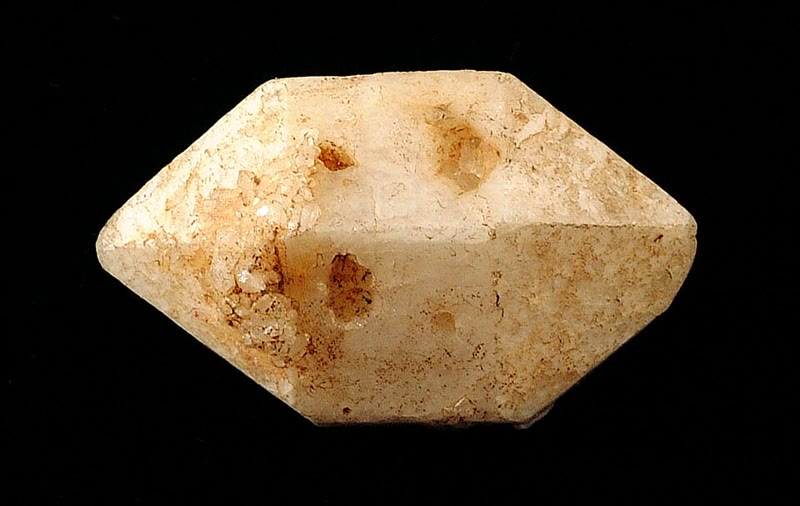
\includegraphics[height=2.75cm]{images/book2/g11-geodil-quartz.jpg}\hfill
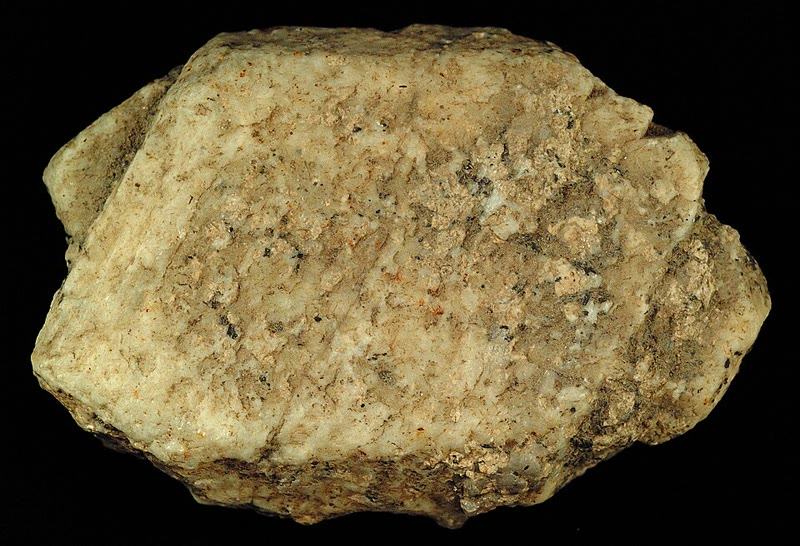
\includegraphics[height=2.75cm]{images/book2/g11-geodil-orthoclase.jpg}\hfill
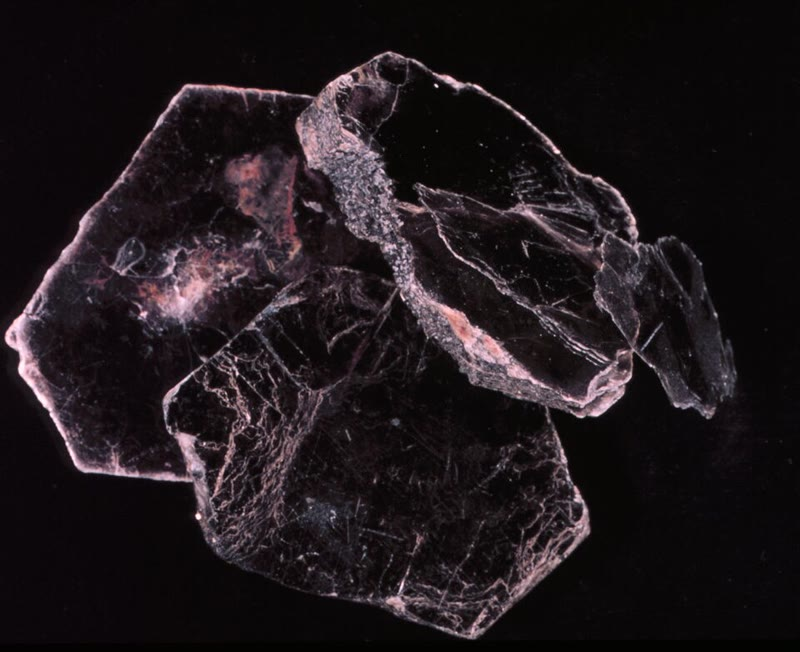
\includegraphics[height=2.75cm]{images/book2/g11-geodil-biotite.jpg}\hfill
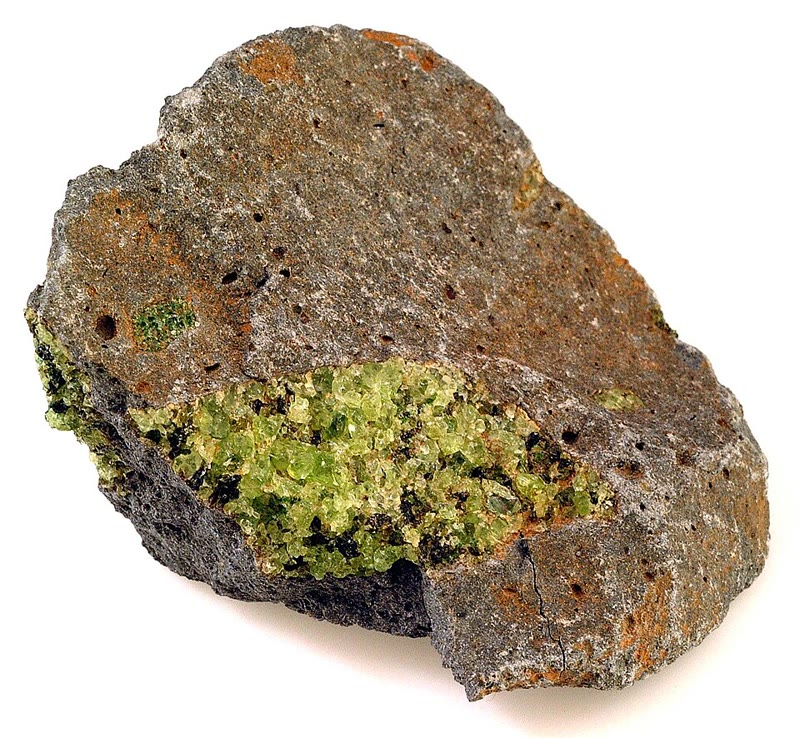
\includegraphics[height=2.75cm]{images/book2/g11-geodil-olivine.jpg}

{\small Quatro minerais formadores de rochas. Da esquerda para a direita: um
cristal de quartzo, um prisma de seis faces terminado em pontas nas duas
extremidades, com cerca de \qty{5}{cm} de comprimento; um feldspato
ortoclásio, dois cristais crescidos juntos, com cerca de \qty{7}{cm}; placas
de seis lados de mica biotita, com cerca de \qty{6}{cm}, que se partem em
folhas finas ao longo da sua única \omterm{def:g11:minerals:cleavage}{clivagem}; grãos verdes de olivina num
basalto. Fotografias Shannon Heinle, Darla Sondrol, Dexter Perkins e Nessa
Eull, Geology Digital Image Library (CC0).}
\end{omfigure}
% ledger: photo:g11-quartz, photo:g11-orthoclase, photo:g11-biotite, photo:g11-olivine

\section{Os silicatos}

\paragraph{Dois elementos formam a crosta.} A composição química da crosta
continental é conhecida pelas análises de muitas rochas, expressas em
porcentagens de óxidos: cerca de \qty{60.6}{\percent} de \ce{SiO2},
\qty{15.9}{\percent} de \ce{Al2O3}, e assim por diante. A partir delas, e das
massas dos átomos, obtém-se a massa de cada elemento. O oxigênio forma
\qty{46}{\percent} da massa da crosta continental e o silício
\qty{28}{\percent}: dois elementos, cerca de três quartos da massa. Com seis
metais --- alumínio, ferro, cálcio, magnésio, sódio e potássio --- eles
formam mais de \qty{99}{\percent} dela.
% ledger: rg14:crust, ciaaw:O, ciaaw:Si, ciaaw:Al, ciaaw:Fe, ciaaw:Ca, ciaaw:Mg, ciaaw:Na, ciaaw:K, ciaaw:Ti, ciaaw:Mn, ciaaw:P
% values (mineral_density.py): bulk_O 46.36, bulk_Si 28.30, O+Si 74.66, eight elements 99.43

\begin{omfigure}
\begin{tikzpicture}
\begin{axis}[omrecord, width=0.82\linewidth, height=5.6cm, ybar, bar width=14pt,
  ymin=0, ymax=55, xtick=data, enlarge x limits=0.06,
  xticklabels from table={figdata/out/grade-11-mineral_density-elements.dat}{symbol},
  ylabel={parte da massa (\unit{\percent})},
  nodes near coords, every node near coord/.append style={font=\scriptsize, /pgf/number format/.cd, fixed, precision=1},
  xmajorgrids=false]
% computed in figdata/grade-11/mineral_density.py; ledger: rg14:crust, ciaaw:*
\addplot[fill=omDef!55, draw=omDef] table[x expr=\coordindex, y=frac] {figdata/out/grade-11-mineral_density-elements.dat};
\end{axis}
\end{tikzpicture}

{\small Os elementos da crosta continental, como partes da sua massa,
calculadas a partir da sua composição média em óxidos (Rudnick e Gao,
2014). O oxigênio e o silício sozinhos formam cerca de três quartos da
massa.}
\end{omfigure}

\paragraph{O tetraedro silício--oxigênio.} Um átomo de silício é pequeno, e
quatro átomos de oxigênio cabem em volta dele, nos vértices de um tetraedro,
uma pirâmide de quatro faces triangulares. O grupo contém um íon silício
\ce{Si^4+} e quatro íons oxigênio \ce{O^2-}: ele carrega uma carga de
$4 - 4 \times 2 = -4$, que outros íons --- ou outros tetraedros --- precisam
equilibrar.

\begin{definition}[Silicato; tetraedro silício--oxigênio]\label{def:g11:minerals:silicate}
O \emph{tetraedro silício--oxigênio}\index{tetraedro silicio--oxigenio@tetraedro silício--oxigênio} é
o grupo \ce{SiO4} formado por um átomo de silício e pelos quatro átomos de
oxigênio em volta dele, nos vértices de um tetraedro. Um
\emph{silicato}\index{silicato} é um mineral construído de tetraedros
silício--oxigênio, isolados ou ligados uns aos outros por vértices
compartilhados.
\end{definition}
% ledger: tulane:silicates

Os tetraedros se ligam compartilhando oxigênios: o vértice de um tetraedro é
o vértice do seguinte. Quantos vértices cada tetraedro compartilha determina
a estrutura do \omterm{def:g11:minerals:silicate}{silicato}, e a sua fórmula.
\begin{itemize}
  \item \emph{Tetraedros isolados}, que não compartilham nenhum vértice,
        mantidos juntos por íons metálicos entre eles: a olivina,
        \ce{(Mg,Fe)2SiO4}.
  \item \emph{Cadeias simples}, cada tetraedro compartilhando dois vértices
        com os seus vizinhos: os piroxênios.
  \item \emph{Cadeias duplas}, duas cadeias simples unidas lado a lado, os
        tetraedros compartilhando alternadamente dois ou três vértices: os
        anfibólios.
  \item \emph{Folhas}, cada tetraedro compartilhando três vértices: as
        micas, e os \omterm{def:g10:soil-formation:clay}{argilominerais} dos solos (\cref{ch:g10:soil-formation}).
  \item \emph{Arcabouços}, cada tetraedro compartilhando os seus quatro
        vértices, nas três direções do espaço: o quartzo, \ce{SiO2}, e --- com
        alumínio no lugar de parte do silício --- os feldspatos.
\end{itemize}
% ledger: tulane:silicates

\begin{omfigure}
\begin{tikzpicture}[font=\footnotesize]
  % coordinates generated once by a small script (scratch, not kept): kagome net of side 0.62 cm,
  % a regular tetrahedron in perspective, and a framework piece of five tetrahedra (painter's order)
  % (a) one SiO4 tetrahedron, drawn in perspective; the silicon (black) at its centre
  \fill[omDef!12] (2.300,2.979) -- (1.927,1.372) -- (1.221,0.629) -- (3.752,0.820) -- cycle;
  \draw[densely dashed, omDef!60, line width=0.6pt] (2.300,2.979) -- (1.927,1.372);
  \draw[omDef!70!black, line width=0.6pt] (2.300,2.979) -- (1.221,0.629);
  \draw[omDef!70!black, line width=0.6pt] (2.300,2.979) -- (3.752,0.820);
  \draw[densely dashed, omDef!60, line width=0.6pt] (1.927,1.372) -- (1.221,0.629);
  \draw[densely dashed, omDef!60, line width=0.6pt] (1.927,1.372) -- (3.752,0.820);
  \draw[omDef!70!black, line width=0.6pt] (1.221,0.629) -- (3.752,0.820);
  \draw[black!55, line width=0.4pt] (2.300,1.450) -- (2.300,2.979);
  \draw[black!55, line width=0.4pt] (2.300,1.450) -- (1.927,1.372);
  \draw[black!55, line width=0.4pt] (2.300,1.450) -- (1.221,0.629);
  \draw[black!55, line width=0.4pt] (2.300,1.450) -- (3.752,0.820);
  \fill[black] (2.300,1.450) circle (2.2pt);
  \filldraw[fill=omThm!35, draw=omThm!80!black, line width=0.4pt] (2.300,2.979) circle (4.2pt);
  \filldraw[fill=omThm!35, draw=omThm!80!black, line width=0.4pt] (1.927,1.372) circle (4.2pt);
  \filldraw[fill=omThm!35, draw=omThm!80!black, line width=0.4pt] (1.221,0.629) circle (4.2pt);
  \filldraw[fill=omThm!35, draw=omThm!80!black, line width=0.4pt] (3.752,0.820) circle (4.2pt);
  % coordinates for labels: Si 2.300,1.450; apex 2.300,2.979
  % (b) isolated tetrahedra (olivine)
  \filldraw[fill=omDef!22, draw=omDef!70!black, line width=0.5pt] (6.200,0.900) -- (6.820,0.900) -- (6.510,1.437) -- cycle;
  \fill[black] (6.510,1.079) circle (0.9pt);
  \filldraw[fill=omDef!22, draw=omDef!70!black, line width=0.5pt] (8.370,1.437) -- (8.990,1.437) -- (8.680,1.974) -- cycle;
  \fill[black] (8.680,1.616) circle (0.9pt);
  \filldraw[fill=omDef!22, draw=omDef!70!black, line width=0.5pt] (8.060,1.974) -- (7.750,2.511) -- (8.370,2.511) -- cycle;
  \fill[black] (8.060,2.332) circle (0.9pt);
  \filldraw[fill=omDef!22, draw=omDef!70!black, line width=0.5pt] (8.990,0.363) -- (9.610,0.363) -- (9.300,0.900) -- cycle;
  \fill[black] (9.300,0.542) circle (0.9pt);
  \filldraw[fill=omDef!22, draw=omDef!70!black, line width=0.5pt] (9.920,1.974) -- (9.610,2.511) -- (10.230,2.511) -- cycle;
  \fill[black] (9.920,2.332) circle (0.9pt);
  \filldraw[fill=omThm!35, draw=omThm!80!black, line width=0.4pt] (6.200,0.900) circle (1.9pt);
  \filldraw[fill=omThm!35, draw=omThm!80!black, line width=0.4pt] (6.510,1.437) circle (1.9pt);
  \filldraw[fill=omThm!35, draw=omThm!80!black, line width=0.4pt] (6.820,0.900) circle (1.9pt);
  \filldraw[fill=omThm!35, draw=omThm!80!black, line width=0.4pt] (7.750,2.511) circle (1.9pt);
  \filldraw[fill=omThm!35, draw=omThm!80!black, line width=0.4pt] (8.060,1.974) circle (1.9pt);
  \filldraw[fill=omThm!35, draw=omThm!80!black, line width=0.4pt] (8.370,2.511) circle (1.9pt);
  \filldraw[fill=omThm!35, draw=omThm!80!black, line width=0.4pt] (8.370,1.437) circle (1.9pt);
  \filldraw[fill=omThm!35, draw=omThm!80!black, line width=0.4pt] (8.680,1.974) circle (1.9pt);
  \filldraw[fill=omThm!35, draw=omThm!80!black, line width=0.4pt] (8.990,1.437) circle (1.9pt);
  \filldraw[fill=omThm!35, draw=omThm!80!black, line width=0.4pt] (9.610,2.511) circle (1.9pt);
  \filldraw[fill=omThm!35, draw=omThm!80!black, line width=0.4pt] (8.990,0.363) circle (1.9pt);
  \filldraw[fill=omThm!35, draw=omThm!80!black, line width=0.4pt] (9.300,0.900) circle (1.9pt);
  \filldraw[fill=omThm!35, draw=omThm!80!black, line width=0.4pt] (9.920,1.974) circle (1.9pt);
  \filldraw[fill=omThm!35, draw=omThm!80!black, line width=0.4pt] (10.230,2.511) circle (1.9pt);
  \filldraw[fill=omThm!35, draw=omThm!80!black, line width=0.4pt] (9.610,0.363) circle (1.9pt);
  % (c) single chain (pyroxenes)
  \filldraw[fill=omDef!22, draw=omDef!70!black, line width=0.5pt] (11.400,1.600) -- (12.020,1.600) -- (11.710,2.137) -- cycle;
  \fill[black] (11.710,1.779) circle (0.9pt);
  \filldraw[fill=omDef!22, draw=omDef!70!black, line width=0.5pt] (12.330,1.063) -- (12.020,1.600) -- (12.640,1.600) -- cycle;
  \fill[black] (12.330,1.421) circle (0.9pt);
  \filldraw[fill=omDef!22, draw=omDef!70!black, line width=0.5pt] (12.640,1.600) -- (13.260,1.600) -- (12.950,2.137) -- cycle;
  \fill[black] (12.950,1.779) circle (0.9pt);
  \filldraw[fill=omDef!22, draw=omDef!70!black, line width=0.5pt] (13.570,1.063) -- (13.260,1.600) -- (13.880,1.600) -- cycle;
  \fill[black] (13.570,1.421) circle (0.9pt);
  \filldraw[fill=omDef!22, draw=omDef!70!black, line width=0.5pt] (13.880,1.600) -- (14.500,1.600) -- (14.190,2.137) -- cycle;
  \fill[black] (14.190,1.779) circle (0.9pt);
  \filldraw[fill=omDef!22, draw=omDef!70!black, line width=0.5pt] (14.810,1.063) -- (14.500,1.600) -- (15.120,1.600) -- cycle;
  \fill[black] (14.810,1.421) circle (0.9pt);
  \filldraw[fill=omDef!22, draw=omDef!70!black, line width=0.5pt] (15.120,1.600) -- (15.740,1.600) -- (15.430,2.137) -- cycle;
  \fill[black] (15.430,1.779) circle (0.9pt);
  \filldraw[fill=omThm!35, draw=omThm!80!black, line width=0.4pt] (11.400,1.600) circle (1.9pt);
  \filldraw[fill=omThm!35, draw=omThm!80!black, line width=0.4pt] (11.710,2.137) circle (1.9pt);
  \filldraw[fill=omThm!35, draw=omThm!80!black, line width=0.4pt] (12.020,1.600) circle (1.9pt);
  \filldraw[fill=omThm!35, draw=omThm!80!black, line width=0.4pt] (12.330,1.063) circle (1.9pt);
  \filldraw[fill=omThm!35, draw=omThm!80!black, line width=0.4pt] (12.640,1.600) circle (1.9pt);
  \filldraw[fill=omThm!35, draw=omThm!80!black, line width=0.4pt] (12.950,2.137) circle (1.9pt);
  \filldraw[fill=omThm!35, draw=omThm!80!black, line width=0.4pt] (13.260,1.600) circle (1.9pt);
  \filldraw[fill=omThm!35, draw=omThm!80!black, line width=0.4pt] (13.570,1.063) circle (1.9pt);
  \filldraw[fill=omThm!35, draw=omThm!80!black, line width=0.4pt] (13.880,1.600) circle (1.9pt);
  \filldraw[fill=omThm!35, draw=omThm!80!black, line width=0.4pt] (14.190,2.137) circle (1.9pt);
  \filldraw[fill=omThm!35, draw=omThm!80!black, line width=0.4pt] (14.500,1.600) circle (1.9pt);
  \filldraw[fill=omThm!35, draw=omThm!80!black, line width=0.4pt] (14.810,1.063) circle (1.9pt);
  \filldraw[fill=omThm!35, draw=omThm!80!black, line width=0.4pt] (15.120,1.600) circle (1.9pt);
  \filldraw[fill=omThm!35, draw=omThm!80!black, line width=0.4pt] (15.430,2.137) circle (1.9pt);
  \filldraw[fill=omThm!35, draw=omThm!80!black, line width=0.4pt] (15.740,1.600) circle (1.9pt);
  % (d) double chain (amphiboles)
  \filldraw[fill=omDef!22, draw=omDef!70!black, line width=0.5pt] (0.600,-3.550) -- (1.220,-3.550) -- (0.910,-3.013) -- cycle;
  \fill[black] (0.910,-3.371) circle (0.9pt);
  \filldraw[fill=omDef!22, draw=omDef!70!black, line width=0.5pt] (1.530,-4.087) -- (1.220,-3.550) -- (1.840,-3.550) -- cycle;
  \fill[black] (1.530,-3.729) circle (0.9pt);
  \filldraw[fill=omDef!22, draw=omDef!70!black, line width=0.5pt] (1.840,-3.550) -- (2.460,-3.550) -- (2.150,-3.013) -- cycle;
  \fill[black] (2.150,-3.371) circle (0.9pt);
  \filldraw[fill=omDef!22, draw=omDef!70!black, line width=0.5pt] (2.770,-4.087) -- (2.460,-3.550) -- (3.080,-3.550) -- cycle;
  \fill[black] (2.770,-3.729) circle (0.9pt);
  \filldraw[fill=omDef!22, draw=omDef!70!black, line width=0.5pt] (3.080,-3.550) -- (3.700,-3.550) -- (3.390,-3.013) -- cycle;
  \fill[black] (3.390,-3.371) circle (0.9pt);
  \filldraw[fill=omDef!22, draw=omDef!70!black, line width=0.5pt] (4.010,-4.087) -- (3.700,-3.550) -- (4.320,-3.550) -- cycle;
  \fill[black] (4.010,-3.729) circle (0.9pt);
  \filldraw[fill=omDef!22, draw=omDef!70!black, line width=0.5pt] (4.320,-3.550) -- (4.940,-3.550) -- (4.630,-3.013) -- cycle;
  \fill[black] (4.630,-3.371) circle (0.9pt);
  \filldraw[fill=omDef!22, draw=omDef!70!black, line width=0.5pt] (0.910,-3.013) -- (0.600,-2.476) -- (1.220,-2.476) -- cycle;
  \fill[black] (0.910,-2.655) circle (0.9pt);
  \filldraw[fill=omDef!22, draw=omDef!70!black, line width=0.5pt] (1.220,-2.476) -- (1.840,-2.476) -- (1.530,-1.939) -- cycle;
  \fill[black] (1.530,-2.297) circle (0.9pt);
  \filldraw[fill=omDef!22, draw=omDef!70!black, line width=0.5pt] (2.150,-3.013) -- (1.840,-2.476) -- (2.460,-2.476) -- cycle;
  \fill[black] (2.150,-2.655) circle (0.9pt);
  \filldraw[fill=omDef!22, draw=omDef!70!black, line width=0.5pt] (2.460,-2.476) -- (3.080,-2.476) -- (2.770,-1.939) -- cycle;
  \fill[black] (2.770,-2.297) circle (0.9pt);
  \filldraw[fill=omDef!22, draw=omDef!70!black, line width=0.5pt] (3.390,-3.013) -- (3.080,-2.476) -- (3.700,-2.476) -- cycle;
  \fill[black] (3.390,-2.655) circle (0.9pt);
  \filldraw[fill=omDef!22, draw=omDef!70!black, line width=0.5pt] (3.700,-2.476) -- (4.320,-2.476) -- (4.010,-1.939) -- cycle;
  \fill[black] (4.010,-2.297) circle (0.9pt);
  \filldraw[fill=omDef!22, draw=omDef!70!black, line width=0.5pt] (4.630,-3.013) -- (4.320,-2.476) -- (4.940,-2.476) -- cycle;
  \fill[black] (4.630,-2.655) circle (0.9pt);
  \filldraw[fill=omThm!35, draw=omThm!80!black, line width=0.4pt] (0.600,-2.476) circle (1.9pt);
  \filldraw[fill=omThm!35, draw=omThm!80!black, line width=0.4pt] (0.600,-3.550) circle (1.9pt);
  \filldraw[fill=omThm!35, draw=omThm!80!black, line width=0.4pt] (0.910,-3.013) circle (1.9pt);
  \filldraw[fill=omThm!35, draw=omThm!80!black, line width=0.4pt] (1.220,-2.476) circle (1.9pt);
  \filldraw[fill=omThm!35, draw=omThm!80!black, line width=0.4pt] (1.530,-1.939) circle (1.9pt);
  \filldraw[fill=omThm!35, draw=omThm!80!black, line width=0.4pt] (1.220,-3.550) circle (1.9pt);
  \filldraw[fill=omThm!35, draw=omThm!80!black, line width=0.4pt] (1.840,-2.476) circle (1.9pt);
  \filldraw[fill=omThm!35, draw=omThm!80!black, line width=0.4pt] (1.530,-4.087) circle (1.9pt);
  \filldraw[fill=omThm!35, draw=omThm!80!black, line width=0.4pt] (1.840,-3.550) circle (1.9pt);
  \filldraw[fill=omThm!35, draw=omThm!80!black, line width=0.4pt] (2.150,-3.013) circle (1.9pt);
  \filldraw[fill=omThm!35, draw=omThm!80!black, line width=0.4pt] (2.460,-2.476) circle (1.9pt);
  \filldraw[fill=omThm!35, draw=omThm!80!black, line width=0.4pt] (2.770,-1.939) circle (1.9pt);
  \filldraw[fill=omThm!35, draw=omThm!80!black, line width=0.4pt] (2.460,-3.550) circle (1.9pt);
  \filldraw[fill=omThm!35, draw=omThm!80!black, line width=0.4pt] (3.080,-2.476) circle (1.9pt);
  \filldraw[fill=omThm!35, draw=omThm!80!black, line width=0.4pt] (2.770,-4.087) circle (1.9pt);
  \filldraw[fill=omThm!35, draw=omThm!80!black, line width=0.4pt] (3.080,-3.550) circle (1.9pt);
  \filldraw[fill=omThm!35, draw=omThm!80!black, line width=0.4pt] (3.390,-3.013) circle (1.9pt);
  \filldraw[fill=omThm!35, draw=omThm!80!black, line width=0.4pt] (3.700,-2.476) circle (1.9pt);
  \filldraw[fill=omThm!35, draw=omThm!80!black, line width=0.4pt] (4.010,-1.939) circle (1.9pt);
  \filldraw[fill=omThm!35, draw=omThm!80!black, line width=0.4pt] (3.700,-3.550) circle (1.9pt);
  \filldraw[fill=omThm!35, draw=omThm!80!black, line width=0.4pt] (4.320,-2.476) circle (1.9pt);
  \filldraw[fill=omThm!35, draw=omThm!80!black, line width=0.4pt] (4.010,-4.087) circle (1.9pt);
  \filldraw[fill=omThm!35, draw=omThm!80!black, line width=0.4pt] (4.320,-3.550) circle (1.9pt);
  \filldraw[fill=omThm!35, draw=omThm!80!black, line width=0.4pt] (4.630,-3.013) circle (1.9pt);
  \filldraw[fill=omThm!35, draw=omThm!80!black, line width=0.4pt] (4.940,-2.476) circle (1.9pt);
  \filldraw[fill=omThm!35, draw=omThm!80!black, line width=0.4pt] (4.940,-3.550) circle (1.9pt);
  % (e) sheet (micas)
  \filldraw[fill=omDef!22, draw=omDef!70!black, line width=0.5pt] (5.900,-4.100) -- (6.520,-4.100) -- (6.210,-3.563) -- cycle;
  \fill[black] (6.210,-3.921) circle (0.9pt);
  \filldraw[fill=omDef!22, draw=omDef!70!black, line width=0.5pt] (7.140,-4.100) -- (7.760,-4.100) -- (7.450,-3.563) -- cycle;
  \fill[black] (7.450,-3.921) circle (0.9pt);
  \filldraw[fill=omDef!22, draw=omDef!70!black, line width=0.5pt] (8.380,-4.100) -- (9.000,-4.100) -- (8.690,-3.563) -- cycle;
  \fill[black] (8.690,-3.921) circle (0.9pt);
  \filldraw[fill=omDef!22, draw=omDef!70!black, line width=0.5pt] (9.620,-4.100) -- (10.240,-4.100) -- (9.930,-3.563) -- cycle;
  \fill[black] (9.930,-3.921) circle (0.9pt);
  \filldraw[fill=omDef!22, draw=omDef!70!black, line width=0.5pt] (6.210,-3.563) -- (5.900,-3.026) -- (6.520,-3.026) -- cycle;
  \fill[black] (6.210,-3.205) circle (0.9pt);
  \filldraw[fill=omDef!22, draw=omDef!70!black, line width=0.5pt] (7.450,-3.563) -- (7.140,-3.026) -- (7.760,-3.026) -- cycle;
  \fill[black] (7.450,-3.205) circle (0.9pt);
  \filldraw[fill=omDef!22, draw=omDef!70!black, line width=0.5pt] (8.690,-3.563) -- (8.380,-3.026) -- (9.000,-3.026) -- cycle;
  \fill[black] (8.690,-3.205) circle (0.9pt);
  \filldraw[fill=omDef!22, draw=omDef!70!black, line width=0.5pt] (9.930,-3.563) -- (9.620,-3.026) -- (10.240,-3.026) -- cycle;
  \fill[black] (9.930,-3.205) circle (0.9pt);
  \filldraw[fill=omDef!22, draw=omDef!70!black, line width=0.5pt] (6.520,-3.026) -- (7.140,-3.026) -- (6.830,-2.489) -- cycle;
  \fill[black] (6.830,-2.847) circle (0.9pt);
  \filldraw[fill=omDef!22, draw=omDef!70!black, line width=0.5pt] (7.760,-3.026) -- (8.380,-3.026) -- (8.070,-2.489) -- cycle;
  \fill[black] (8.070,-2.847) circle (0.9pt);
  \filldraw[fill=omDef!22, draw=omDef!70!black, line width=0.5pt] (9.000,-3.026) -- (9.620,-3.026) -- (9.310,-2.489) -- cycle;
  \fill[black] (9.310,-2.847) circle (0.9pt);
  \filldraw[fill=omDef!22, draw=omDef!70!black, line width=0.5pt] (6.830,-2.489) -- (6.520,-1.952) -- (7.140,-1.952) -- cycle;
  \fill[black] (6.830,-2.131) circle (0.9pt);
  \filldraw[fill=omDef!22, draw=omDef!70!black, line width=0.5pt] (8.070,-2.489) -- (7.760,-1.952) -- (8.380,-1.952) -- cycle;
  \fill[black] (8.070,-2.131) circle (0.9pt);
  \filldraw[fill=omDef!22, draw=omDef!70!black, line width=0.5pt] (9.310,-2.489) -- (9.000,-1.952) -- (9.620,-1.952) -- cycle;
  \fill[black] (9.310,-2.131) circle (0.9pt);
  \filldraw[fill=omDef!22, draw=omDef!70!black, line width=0.5pt] (5.900,-1.952) -- (6.520,-1.952) -- (6.210,-1.415) -- cycle;
  \fill[black] (6.210,-1.773) circle (0.9pt);
  \filldraw[fill=omDef!22, draw=omDef!70!black, line width=0.5pt] (7.140,-1.952) -- (7.760,-1.952) -- (7.450,-1.415) -- cycle;
  \fill[black] (7.450,-1.773) circle (0.9pt);
  \filldraw[fill=omDef!22, draw=omDef!70!black, line width=0.5pt] (8.380,-1.952) -- (9.000,-1.952) -- (8.690,-1.415) -- cycle;
  \fill[black] (8.690,-1.773) circle (0.9pt);
  \filldraw[fill=omDef!22, draw=omDef!70!black, line width=0.5pt] (9.620,-1.952) -- (10.240,-1.952) -- (9.930,-1.415) -- cycle;
  \fill[black] (9.930,-1.773) circle (0.9pt);
  \filldraw[fill=omThm!35, draw=omThm!80!black, line width=0.4pt] (5.900,-1.952) circle (1.9pt);
  \filldraw[fill=omThm!35, draw=omThm!80!black, line width=0.4pt] (6.210,-1.415) circle (1.9pt);
  \filldraw[fill=omThm!35, draw=omThm!80!black, line width=0.4pt] (5.900,-3.026) circle (1.9pt);
  \filldraw[fill=omThm!35, draw=omThm!80!black, line width=0.4pt] (6.520,-1.952) circle (1.9pt);
  \filldraw[fill=omThm!35, draw=omThm!80!black, line width=0.4pt] (5.900,-4.100) circle (1.9pt);
  \filldraw[fill=omThm!35, draw=omThm!80!black, line width=0.4pt] (6.210,-3.563) circle (1.9pt);
  \filldraw[fill=omThm!35, draw=omThm!80!black, line width=0.4pt] (6.520,-3.026) circle (1.9pt);
  \filldraw[fill=omThm!35, draw=omThm!80!black, line width=0.4pt] (6.830,-2.489) circle (1.9pt);
  \filldraw[fill=omThm!35, draw=omThm!80!black, line width=0.4pt] (7.140,-1.952) circle (1.9pt);
  \filldraw[fill=omThm!35, draw=omThm!80!black, line width=0.4pt] (7.450,-1.415) circle (1.9pt);
  \filldraw[fill=omThm!35, draw=omThm!80!black, line width=0.4pt] (6.520,-4.100) circle (1.9pt);
  \filldraw[fill=omThm!35, draw=omThm!80!black, line width=0.4pt] (7.140,-3.026) circle (1.9pt);
  \filldraw[fill=omThm!35, draw=omThm!80!black, line width=0.4pt] (7.760,-1.952) circle (1.9pt);
  \filldraw[fill=omThm!35, draw=omThm!80!black, line width=0.4pt] (7.140,-4.100) circle (1.9pt);
  \filldraw[fill=omThm!35, draw=omThm!80!black, line width=0.4pt] (7.450,-3.563) circle (1.9pt);
  \filldraw[fill=omThm!35, draw=omThm!80!black, line width=0.4pt] (7.760,-3.026) circle (1.9pt);
  \filldraw[fill=omThm!35, draw=omThm!80!black, line width=0.4pt] (8.070,-2.489) circle (1.9pt);
  \filldraw[fill=omThm!35, draw=omThm!80!black, line width=0.4pt] (8.380,-1.952) circle (1.9pt);
  \filldraw[fill=omThm!35, draw=omThm!80!black, line width=0.4pt] (8.690,-1.415) circle (1.9pt);
  \filldraw[fill=omThm!35, draw=omThm!80!black, line width=0.4pt] (7.760,-4.100) circle (1.9pt);
  \filldraw[fill=omThm!35, draw=omThm!80!black, line width=0.4pt] (8.380,-3.026) circle (1.9pt);
  \filldraw[fill=omThm!35, draw=omThm!80!black, line width=0.4pt] (9.000,-1.952) circle (1.9pt);
  \filldraw[fill=omThm!35, draw=omThm!80!black, line width=0.4pt] (8.380,-4.100) circle (1.9pt);
  \filldraw[fill=omThm!35, draw=omThm!80!black, line width=0.4pt] (8.690,-3.563) circle (1.9pt);
  \filldraw[fill=omThm!35, draw=omThm!80!black, line width=0.4pt] (9.000,-3.026) circle (1.9pt);
  \filldraw[fill=omThm!35, draw=omThm!80!black, line width=0.4pt] (9.310,-2.489) circle (1.9pt);
  \filldraw[fill=omThm!35, draw=omThm!80!black, line width=0.4pt] (9.620,-1.952) circle (1.9pt);
  \filldraw[fill=omThm!35, draw=omThm!80!black, line width=0.4pt] (9.930,-1.415) circle (1.9pt);
  \filldraw[fill=omThm!35, draw=omThm!80!black, line width=0.4pt] (9.000,-4.100) circle (1.9pt);
  \filldraw[fill=omThm!35, draw=omThm!80!black, line width=0.4pt] (9.620,-3.026) circle (1.9pt);
  \filldraw[fill=omThm!35, draw=omThm!80!black, line width=0.4pt] (10.240,-1.952) circle (1.9pt);
  \filldraw[fill=omThm!35, draw=omThm!80!black, line width=0.4pt] (9.620,-4.100) circle (1.9pt);
  \filldraw[fill=omThm!35, draw=omThm!80!black, line width=0.4pt] (9.930,-3.563) circle (1.9pt);
  \filldraw[fill=omThm!35, draw=omThm!80!black, line width=0.4pt] (10.240,-3.026) circle (1.9pt);
  \filldraw[fill=omThm!35, draw=omThm!80!black, line width=0.4pt] (10.240,-4.100) circle (1.9pt);
  % (f) framework: a tetrahedron sharing all four corners
  \filldraw[fill=omThm!35, draw=omThm!80!black, line width=0.4pt] (12.990,-1.963) circle (2.1pt);
  \filldraw[fill=omThm!35, draw=omThm!80!black, line width=0.4pt] (12.896,-3.062) circle (2.1pt);
  \filldraw[fill=omDef!14, draw=omDef!70!black, line width=0.45pt, fill opacity=0.85] (12.896,-3.062) -- (12.990,-1.963) -- (12.299,-2.380) -- cycle;
  \filldraw[fill=omThm!35, draw=omThm!80!black, line width=0.4pt] (15.186,-2.119) circle (2.1pt);
  \filldraw[fill=omDef!14, draw=omDef!70!black, line width=0.45pt, fill opacity=0.85] (12.896,-3.062) -- (13.398,-2.458) -- (12.990,-1.963) -- cycle;
  \filldraw[fill=omThm!35, draw=omThm!80!black, line width=0.4pt] (15.092,-3.219) circle (2.1pt);
  \fill[black] (12.896,-2.466) circle (1.1pt);
  \filldraw[fill=omDef!34, draw=omDef!70!black, line width=0.45pt, fill opacity=0.85] (13.398,-2.458) -- (12.990,-1.963) -- (12.299,-2.380) -- cycle;
  \filldraw[fill=omDef!14, draw=omDef!70!black, line width=0.45pt, fill opacity=0.85] (15.092,-3.219) -- (15.186,-2.119) -- (14.496,-2.536) -- cycle;
  \filldraw[fill=omDef!25, draw=omDef!70!black, line width=0.45pt, fill opacity=0.85] (12.896,-3.062) -- (12.299,-2.380) -- (13.398,-2.458) -- cycle;
  \filldraw[fill=omDef!14, draw=omDef!70!black, line width=0.45pt, fill opacity=0.85] (15.092,-3.219) -- (15.595,-2.614) -- (15.186,-2.119) -- cycle;
  \fill[black] (15.092,-2.622) circle (1.1pt);
  \filldraw[fill=omThm!35, draw=omThm!80!black, line width=0.4pt] (12.299,-2.380) circle (2.1pt);
  \filldraw[fill=omDef!34, draw=omDef!70!black, line width=0.45pt, fill opacity=0.85] (15.595,-2.614) -- (15.186,-2.119) -- (14.496,-2.536) -- cycle;
  \filldraw[fill=omDef!25, draw=omDef!70!black, line width=0.45pt, fill opacity=0.85] (15.092,-3.219) -- (14.496,-2.536) -- (15.595,-2.614) -- cycle;
  \filldraw[fill=omThm!35, draw=omThm!80!black, line width=0.4pt] (13.398,-2.458) circle (2.1pt);
  \filldraw[fill=omThm!35, draw=omThm!80!black, line width=0.4pt] (14.496,-2.536) circle (2.1pt);
  \filldraw[fill=omDef!14, draw=omDef!70!black, line width=0.45pt, fill opacity=0.85] (13.900,-1.853) -- (14.496,-2.536) -- (13.398,-2.458) -- cycle;
  \filldraw[fill=omThm!35, draw=omThm!80!black, line width=0.4pt] (15.595,-2.614) circle (2.1pt);
  \filldraw[fill=omDef!14, draw=omDef!70!black, line width=0.45pt, fill opacity=0.85] (13.398,-2.458) -- (13.806,-2.953) -- (14.496,-2.536) -- cycle;
  \fill[black] (13.900,-2.450) circle (1.1pt);
  \filldraw[fill=omDef!22, draw=omDef!70!black, line width=0.45pt, fill opacity=0.85] (13.900,-1.853) -- (13.398,-2.458) -- (13.806,-2.953) -- cycle;
  \filldraw[fill=omDef!37, draw=omDef!70!black, line width=0.45pt, fill opacity=0.85] (13.900,-1.853) -- (13.806,-2.953) -- (14.496,-2.536) -- cycle;
  \filldraw[fill=omThm!35, draw=omThm!80!black, line width=0.4pt] (13.994,-0.754) circle (2.1pt);
  \filldraw[fill=omThm!35, draw=omThm!80!black, line width=0.4pt] (13.900,-1.853) circle (2.1pt);
  \filldraw[fill=omThm!35, draw=omThm!80!black, line width=0.4pt] (13.806,-2.953) circle (2.1pt);
  \filldraw[fill=omDef!14, draw=omDef!70!black, line width=0.45pt, fill opacity=0.85] (13.900,-1.853) -- (13.994,-0.754) -- (13.304,-1.171) -- cycle;
  \filldraw[fill=omDef!14, draw=omDef!70!black, line width=0.45pt, fill opacity=0.85] (13.900,-1.853) -- (14.402,-1.249) -- (13.994,-0.754) -- cycle;
  \filldraw[fill=omThm!35, draw=omThm!80!black, line width=0.4pt] (13.712,-4.053) circle (2.1pt);
  \fill[black] (13.900,-1.256) circle (1.1pt);
  \filldraw[fill=omDef!14, draw=omDef!70!black, line width=0.45pt, fill opacity=0.85] (13.712,-4.053) -- (13.806,-2.953) -- (13.116,-3.370) -- cycle;
  \filldraw[fill=omDef!34, draw=omDef!70!black, line width=0.45pt, fill opacity=0.85] (14.402,-1.249) -- (13.994,-0.754) -- (13.304,-1.171) -- cycle;
  \filldraw[fill=omDef!14, draw=omDef!70!black, line width=0.45pt, fill opacity=0.85] (13.712,-4.053) -- (14.214,-3.448) -- (13.806,-2.953) -- cycle;
  \filldraw[fill=omDef!25, draw=omDef!70!black, line width=0.45pt, fill opacity=0.85] (13.900,-1.853) -- (13.304,-1.171) -- (14.402,-1.249) -- cycle;
  \fill[black] (13.712,-3.456) circle (1.1pt);
  \filldraw[fill=omThm!35, draw=omThm!80!black, line width=0.4pt] (13.304,-1.171) circle (2.1pt);
  \filldraw[fill=omDef!34, draw=omDef!70!black, line width=0.45pt, fill opacity=0.85] (14.214,-3.448) -- (13.806,-2.953) -- (13.116,-3.370) -- cycle;
  \filldraw[fill=omDef!25, draw=omDef!70!black, line width=0.45pt, fill opacity=0.85] (13.712,-4.053) -- (13.116,-3.370) -- (14.214,-3.448) -- cycle;
  \filldraw[fill=omThm!35, draw=omThm!80!black, line width=0.4pt] (14.402,-1.249) circle (2.1pt);
  \filldraw[fill=omThm!35, draw=omThm!80!black, line width=0.4pt] (13.116,-3.370) circle (2.1pt);
  \filldraw[fill=omThm!35, draw=omThm!80!black, line width=0.4pt] (14.214,-3.448) circle (2.1pt);
  % labels
  \draw[black!60] (2.30,2.98) -- (3.35,3.25); \node[anchor=west] at (3.35,3.25) {oxigênio};
  \draw[black!60] (2.30,1.45) -- (3.55,2.15); \node[anchor=west] at (3.55,2.15) {silício};
  \node[align=center] at (2.3,-0.15) {(a) um tetraedro, \ce{SiO4}};
  \node[align=center] at (8.2,-0.15) {(b) tetraedros isolados:\\olivina};
  \node[align=center] at (13.5,-0.15) {(c) cadeia simples:\\piroxênios};
  \node[align=center] at (2.75,-4.85) {(d) cadeia dupla:\\anfibólios};
  \node[align=center] at (8.1,-4.85) {(e) folha:\\micas};
  \node[align=center] at (13.9,-4.85) {(f) arcabouço:\\quartzo, feldspatos};
\end{tikzpicture}

{\small (a) O \omterm{def:g11:minerals:silicate}{tetraedro silício--oxigênio}: um átomo de silício (preto) e
quatro átomos de oxigênio (rosa) nos vértices de um tetraedro. (b)--(e)
Tetraedros vistos de cima, cada um como um triângulo: os círculos são os
oxigênios da sua base, o ponto é o silício, sob o quarto oxigênio; dois
triângulos que se tocam num vértice compartilham esse oxigênio. (f) Num
arcabouço, todos os vértices são compartilhados, em três dimensões: aqui, um
tetraedro e os seus quatro vizinhos. Desenhos fora de escala.}
\end{omfigure}
% ledger: tulane:silicates

\begin{proposition}[Contar os oxigênios]\label{prop:g11:minerals:sharing}
Num \omterm{def:g11:minerals:silicate}{silicato} em que cada tetraedro compartilha $n$ dos seus vértices com
outros tetraedros, há $4 - n/2$ átomos de oxigênio para cada átomo de
silício. Os tetraedros isolados dão \ce{SiO4}, as cadeias simples
\ce{SiO3}, as folhas \ce{Si2O5} e os arcabouços \ce{SiO2}.
\end{proposition}

\begin{proof}
Cada tetraedro tem um silício e quatro vértices. Um vértice que não é
compartilhado pertence só a esse tetraedro e conta como um oxigênio; um
vértice compartilhado pertence a dois tetraedros e conta como meio oxigênio
em cada um. Com $n$ vértices compartilhados, um tetraedro possui
$(4 - n) + n/2 = 4 - n/2$ oxigênios. Para $n = 0$, $2$, $3$ e $4$, isso dá
$4$, $3$, $5/2$ e $2$ oxigênios por silício: \ce{SiO4}, \ce{SiO3},
\ce{Si2O5} e \ce{SiO2}.
\end{proof}

As fórmulas dos minerais confirmam isso. O piroxênio augita contém
\ce{(Si,Al)2O6}, isto é, \ce{SiO3} duas vezes, e a mica biotita
\ce{AlSi3O10}, quatro tetraedros para dez oxigênios, \ce{Si2O5} duas vezes;
num feldspato, quatro tetraedros contêm oito oxigênios, \ce{SiO2} quatro
vezes, exatamente como no quartzo. As cargas, porém, diferem. O quartzo é
neutro: num arcabouço, cada oxigênio é compartilhado, e as cargas do silício
e do oxigênio se equilibram. Nas outras estruturas, os oxigênios não
compartilhados carregam cargas negativas sobrando, equilibradas por íons
metálicos --- magnésio e ferro na olivina, potássio no ortoclásio, onde um
íon alumínio \ce{Al^3+} no lugar de um íon silício \ce{Si^4+} deixa uma
carga a ser equilibrada.
% ledger: wm:densities (formulas)

\begin{definition}[Silicatos formadores de rochas]\label{def:g11:minerals:rock-forming}
Os \emph{silicatos formadores de rochas}\index{silicatos formadores de rochas}
são os seis grupos de minerais silicatados que formam a maior parte das
rochas ígneas e metamórficas comuns: a olivina, os piroxênios, os
anfibólios, as micas, os feldspatos e o quartzo. Os feldspatos são de dois
tipos: o \emph{feldspato potássico}, como o ortoclásio, e o
\emph{plagioclásio}, uma série de feldspatos que contêm sódio e cálcio.
\end{definition}
% ledger: tulane:silicates, wm:densities

\begin{center}
\small
\renewcommand{\arraystretch}{1.25}
\begin{tabular}{|l|l|l|c|}
\hline
\textbf{grupo (exemplo)} & \textbf{estrutura} & \textbf{fórmula} & \textbf{densidade} \\
 & & & (\unit{g/cm^3}) \\
\hline
olivina & tetraedros isolados & \ce{(Mg,Fe)2SiO4} & 3.32 \\
piroxênio (augita) & cadeias simples & \ce{(Ca,Na)(Mg,Fe,Al,Ti)(Si,Al)2O6} & 3.4 \\
anfibólio (hornblenda) & cadeias duplas & \ce{Ca2[Mg4(Al,Fe)]Si7AlO22(OH)2} & 3.23 \\
mica (biotita) & folhas & \ce{K(Mg,Fe)3AlSi3O10(OH,F)2} & 3.09 \\
mica (muscovita) & folhas & \ce{KAl2(Si3Al)O10(OH,F)2} & 2.82 \\
feldspato potássico (ortoclásio) & arcabouço & \ce{KAlSi3O8} & 2.56 \\
plagioclásio (oligoclásio) & arcabouço & \ce{(Na,Ca)(Si,Al)4O8} & 2.65 \\
quartzo & arcabouço & \ce{SiO2} & 2.62 \\
\hline
\end{tabular}

\smallskip
{\footnotesize Os \omterm{def:g11:minerals:rock-forming}{silicatos formadores de rochas}. Fórmulas e densidades
médias de webmineral.com; uma vírgula entre dois elementos entre parênteses
indica que qualquer um deles pode ocupar esse lugar no cristal.}
\end{center}
% ledger: wm:densities, tulane:silicates

A tabela contém uma regra que atravessa o resto deste livro. Os minerais de
tetraedros isolados e de cadeias, ricos em ferro e magnésio, são os mais
densos, acima de \qty{3.2}{g/cm^3}; os arcabouços, feitos de silício,
alumínio, sódio, potássio e cálcio, são os mais leves, cerca de
\qty{2.6}{g/cm^3}. As micas ficam no meio. A olivina e o piroxênio formam o
\omterm{def:g11:ocean-ridges:peridotite}{peridotito} do manto; os feldspatos e o quartzo, o granito dos continentes: a
rocha leve flutua sobre a densa.
% ledger: wm:densities

\section{Os minerais formam as rochas}

Uma rocha é descrita em primeiro lugar pelos seus minerais e pelas suas
proporções. Três rochas vistas em capítulos anteriores mostram a variedade:
\begin{itemize}
  \item o \emph{granito}: quartzo, feldspato potássico e plagioclásio, com um
        pouco de biotita ou de muscovita --- a rocha dos continentes;
  \item o \emph{basalto} e o \emph{\omterm{def:g11:ocean-ridges:gabbro}{gabro}}: plagioclásio e piroxênio, muitas
        vezes com olivina --- as rochas da \omterm{def:g11:ocean-ridges:oceanic-lithosphere}{crosta oceânica}, a primeira de
        grão fino, a segunda de grão grosso (\cref{ch:g11:igneous-rocks});
  \item o \emph{\omterm{def:g11:ocean-ridges:peridotite}{peridotito}}: principalmente olivina, com piroxênio --- a
        rocha do manto.
\end{itemize}
% ledger: nps:granite-minerals, photo:g11-basalt-thin-section, photo:g11-olivine

\begin{omfigure}
\begin{tikzpicture}
\begin{axis}[omrecord, width=0.8\linewidth, height=6.4cm, xbar, bar width=8pt,
  xmin=2.4, xmax=3.5, ymin=-0.7, ymax=8.7, ytick={0,...,8},
  yticklabels={ortoclásio, quartzo, oligoclásio, labradorita, muscovita, biotita, hornblenda, olivina, augita},
  xlabel={densidade (\unit{g/cm^3})}, ymajorgrids=false, clip=false]
% computed in figdata/grade-11/mineral_density.py (density_order); ledger: wm:densities
\addplot[fill=omDef!45, draw=omDef] table[x=rho, y=idx] {figdata/out/grade-11-mineral_density-densities.dat};
\draw[omProp, line width=1pt, dashed] (axis cs:2.6427,-0.7) -- (axis cs:2.6427,8.7) node[above, text height=1.6ex, text depth=0.3ex, font=\scriptsize, text=omProp!80!black] {granito};
\draw[omThm, line width=1pt, dashed] (axis cs:3.0015,-0.7) -- (axis cs:3.0015,8.7) node[above, text height=1.6ex, text depth=0.3ex, font=\scriptsize, text=omThm] {basalto};
\draw[black!70, line width=1pt, dashed] (axis cs:3.34,-0.7) -- (axis cs:3.34,8.7) node[above, font=\scriptsize] {peridotito};
\end{axis}
\end{tikzpicture}

{\small As densidades médias de nove minerais formadores de rochas
(webmineral.com), e as densidades das três rochas de exemplo desta seção
calculadas com a proposição abaixo (linhas tracejadas): um granito de
quartzo, feldspatos e micas, um basalto de plagioclásio, piroxênio e um
pouco de olivina, um \omterm{def:g11:ocean-ridges:peridotite}{peridotito} de olivina e piroxênio.}
\end{omfigure}
% values (mineral_density.py): rho_granite 2.6427, rho_basalt 3.0015, rho_peridotite 3.34

A densidade de uma rocha decorre dos seus minerais. Imagine um bloco de
rocha de volume $V$, uma fração $\phi_1$ dele feita de um primeiro mineral,
$\phi_2$ de um segundo, e assim por diante.

\begin{proposition}[A densidade de uma rocha a partir dos seus minerais]\label{prop:g11:minerals:density}
Uma rocha sem poros, feita de minerais de densidades $\rho_1, \rho_2, \dots,
\rho_k$ que ocupam as frações $\phi_1, \phi_2, \dots, \phi_k$ do seu volume
($\phi_1 + \dots + \phi_k = 1$), tem a densidade
\[
  \rho = \phi_1 \rho_1 + \phi_2 \rho_2 + \dots + \phi_k \rho_k ,
\]
a média das densidades dos seus minerais, ponderada pelas suas frações de
volume.
\end{proposition}

\begin{proof}
Num volume $V$ de rocha, o mineral $i$ ocupa o volume $\phi_i V$ e tem a
massa $\rho_i \phi_i V$. Sem poros, a massa da rocha é a soma dessas
massas, $m = (\phi_1 \rho_1 + \dots + \phi_k \rho_k)\,V$, e a sua
densidade é $m/V$.
\end{proof}

Como se medem as frações de volume? Numa face plana cortada da rocha, ou
numa \omterm{def:g11:minerals:thin-section}{lâmina delgada} (próxima seção), dispõe-se uma grade regular de pontos,
e em cada ponto anota-se o mineral que está embaixo. Quando os grãos estão
espalhados sem ordem, a fração dos pontos que caem sobre um mineral estima a
fração da área que ele cobre, e esta é também a fração do volume que ele
ocupa: uma fatia fina é uma amostra justa do bloco inteiro. É uma
\emph{contagem de pontos}.

\begin{example}[Um granito leve, rico em quartzo e em feldspato potássico]
Uma contagem de pontos dá \qty{35}{\percent} de quartzo (\qty{2.62}{g/cm^3}),
\qty{50}{\percent} de ortoclásio (\qty{2.56}{g/cm^3}) e \qty{15}{\percent}
de oligoclásio (\qty{2.65}{g/cm^3}). A densidade da rocha é
\[
  \rho = 0.35 \times 2.62 + 0.50 \times 2.56 + 0.15 \times 2.65
       = 0.917 + 1.280 + 0.398 \approx \qty{2.59}{g/cm^3}.
\]
As medições confirmam essa ordem de grandeza: de \num{6454} amostras de
rocha pesadas de cerca de duzentos corpos de rocha granítica da Sierra
Nevada, na Califórnia, a média é \qty{2.69}{g/cm^3}, e os granitos mais
ricos em sílica e potássio, como este, ficam abaixo de \qty{2.6}{g/cm^3}.
\end{example}
% ledger: wm:densities, usgs91:sierra

\section{As lâminas delgadas}

Uma lupa mostra grãos de um milímetro. Para ver grãos mais finos, e
identificá-los com certeza, os geólogos olham as rochas ao microscópio ---
não a sua superfície, mas através delas.

\begin{definition}[Lâmina delgada; microscópio de luz polarizada]\label{def:g11:minerals:thin-section}
Uma \emph{lâmina delgada}\index{lamina delgada@lâmina delgada} é uma fatia de
rocha desgastada até uma espessura de \qty{0.03}{mm} e montada numa lâmina
de vidro: nessa espessura, a luz atravessa a maioria dos minerais. Um
\emph{microscópio de luz polarizada}\index{microscopio de luz polarizada@microscópio de luz polarizada}
é um microscópio equipado com dois filtros polarizadores, um abaixo da
lâmina e outro acima. A lâmina é vista em \emph{luz polarizada plana} só com
o filtro inferior, e entre \emph{polarizadores cruzados} quando se acrescenta
o filtro superior com a sua direção perpendicular à do inferior.
\end{definition}
% ledger: tulane:thin-section

\begin{omfigure}
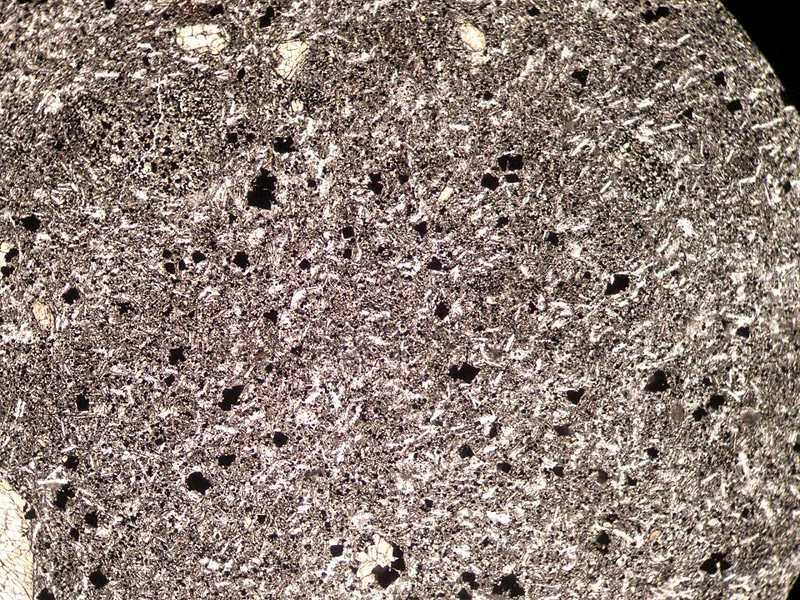
\includegraphics[height=3.6cm]{images/book2/g11-chmee2-basalt-ppl.jpg}\hfill
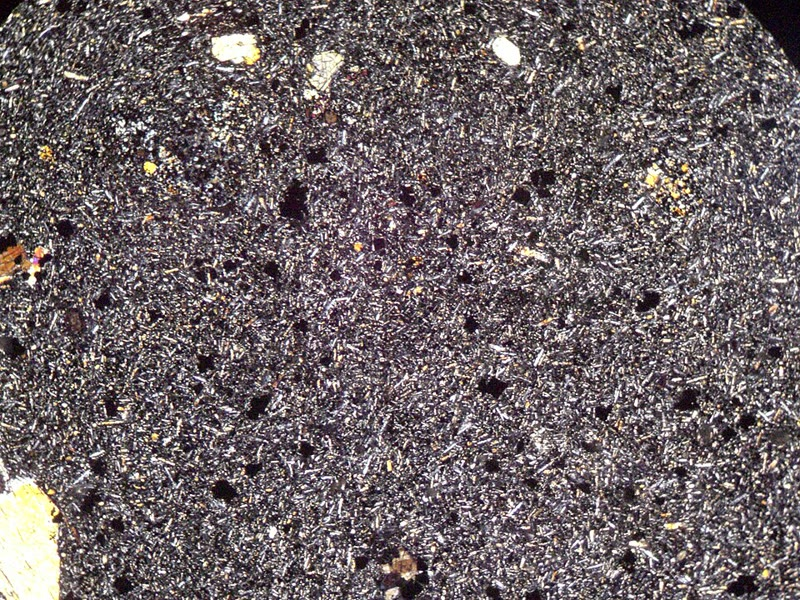
\includegraphics[height=3.6cm]{images/book2/g11-chmee2-basalt-xpl.jpg}\hfill
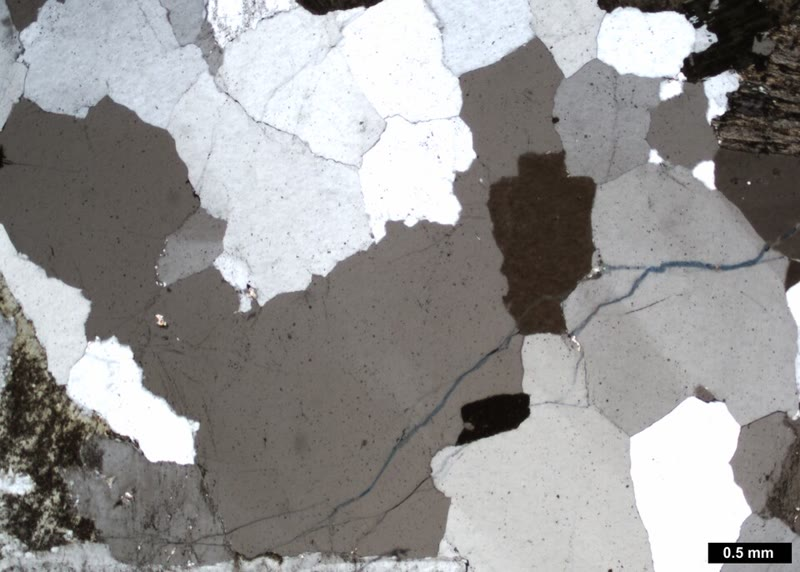
\includegraphics[height=3.6cm]{images/book2/g11-rygel-granite-xpl.jpg}

{\small À esquerda e no centro: o mesmo basalto em \omterm{def:g11:minerals:thin-section}{lâmina delgada}, em luz
polarizada plana e entre polarizadores cruzados. A rocha é de grão fino:
pequenos cristais alongados, principalmente de plagioclásio, e pontos pretos
que não deixam passar nenhuma luz em nenhuma das vistas; entre
polarizadores cruzados, os cristais se acendem em cinzas e em cores. Fotografias
Chmee2 (CC~BY-SA~3.0). À direita: cristais de quartzo num granito, entre
polarizadores cruzados, cada um no seu próprio tom de cinza (a barra de
escala mede \qty{0.5}{mm}). Fotografia Michael C.~Rygel (CC~BY-SA~3.0).}
\end{omfigure}
% ledger: photo:g11-basalt-thin-section, photo:g11-granite-thin-section

Em luz polarizada plana, uma \omterm{def:g11:minerals:thin-section}{lâmina delgada} parece um vitral: a maioria dos
minerais é quase incolor, alguns são tingidos, e os contornos dos grãos, as
suas clivagens e os seus \omterm{def:g11:minerals:habit}{hábitos} aparecem com nitidez. Entre polarizadores
cruzados, os filtros, dispostos um atravessado ao outro, não deixariam
passar luz nenhuma sozinhos; a maioria dos minerais altera a luz que os
atravessa, e aparece em tons de cinza ou em cores vivas, que mudam quando se
gira a lâmina. Dois grãos do mesmo mineral podem parecer diferentes, porque
cada um está cortado na sua própria direção: os grãos de quartzo do granito
acima são todos de quartzo, em tons diferentes. As cores, como elas mudam e
o que revelam sobre cada mineral são assunto do primeiro ano da
universidade; aqui, a \omterm{def:g11:minerals:thin-section}{lâmina delgada} é uma imagem da rocha, na qual cada
grão pode ser visto, nomeado e contado.

\section{Exercícios}

\begin{exercise}[$\star$]\label{exo:g11:minerals:1}
Defina a \omterm{def:g11:minerals:cleavage}{clivagem} e a \omterm{def:g11:minerals:cleavage}{fratura}. Qual das duas o quartzo mostra, e qual é o
aspecto das suas superfícies quebradas? Quantas clivagens tem uma mica?
\end{exercise}

\begin{exercise}[$\star$]\label{exo:g11:minerals:2}
Por que a cor é um mau guia para identificar o quartzo, mas um guia
razoavelmente bom para a olivina? Dê duas propriedades mais confiáveis que a
cor.
\end{exercise}

\begin{exercise}[$\star$]\label{exo:g11:minerals:3}
Associe cada descrição a um mineral entre quartzo, ortoclásio, biotita e
olivina: (1) grãos verdes num basalto; (2) lamelas pretas que se desfolham em
folhas finas; (3) grãos cor-de-rosa, em blocos, com dois planos de ruptura
planos, riscados por um prego de aço; (4) grãos cinzentos e vítreos, com
quebras curvas, não riscados pelo prego.
\end{exercise}

\begin{exercise}[$\star$]\label{exo:g11:minerals:4}
(1) Quantos átomos um \omterm{def:g11:minerals:silicate}{tetraedro silício--oxigênio} contém, e onde ficam?
(2) Usando as cargas dos íons \ce{Si^4+} e \ce{O^2-}, encontre a carga do
grupo \ce{SiO4}.
\end{exercise}

\begin{exercise}[$\star$]\label{exo:g11:minerals:5}
Cite os seis grupos de \omterm{def:g11:minerals:rock-forming}{silicatos formadores de rochas} e dê, para cada um, o
modo como os seus tetraedros estão ligados.
\end{exercise}

\begin{exercise}[$\star\star$]\label{exo:g11:minerals:6}
As massas atômicas do silício e do oxigênio são \qty{28.085}{g/mol} e
\qty{15.999}{g/mol}. (1) Calcule a parte do oxigênio na massa do quartzo,
\ce{SiO2}. (2) Faça o mesmo para a forsterita, a olivina magnesiana
\ce{Mg2SiO4} (magnésio: \qty{24.305}{g/mol}). (3) Compare com a parte do
oxigênio na crosta continental, cerca de \qty{46}{\percent}.
\end{exercise}

\begin{exercise}[$\star\star$]\label{exo:g11:minerals:7}
Um grão branco num granito risca uma placa de vidro (cerca de 5.5), mas é
riscado por um prego de aço (cerca de 6.5); ele se quebra ao longo de
planos em duas direções. Um segundo grão, cinzento, não é riscado pelo prego
e se quebra ao longo de superfícies curvas. Identifique os dois, dando as
razões.
\end{exercise}

\begin{exercise}[$\star\star$]\label{exo:g11:minerals:8}
No piroxênio augita, cada tetraedro compartilha dois vértices. (1) Usando a
proposição sobre a contagem dos oxigênios, quantos oxigênios há para cada
silício? (2) Verifique que a parte \ce{(Si,Al)2O6} da fórmula da augita
concorda.
\end{exercise}

\begin{exercise}[$\star\star$]\label{exo:g11:minerals:9}
Um basalto é feito de \qty{55}{\percent} de labradorita (\qty{2.69}{g/cm^3}),
\qty{35}{\percent} de augita (\qty{3.4}{g/cm^3}) e \qty{10}{\percent} de
olivina (\qty{3.32}{g/cm^3}), em volume. Calcule a sua densidade, e depois a
massa de um cubo desse basalto com \qty{10}{cm} de aresta.
\end{exercise}

\begin{exercise}[$\star\star$]\label{exo:g11:minerals:10}
Um \omterm{def:g11:ocean-ridges:peridotite}{peridotito} do manto é feito de \qty{75}{\percent} de olivina
(\qty{3.32}{g/cm^3}) e \qty{25}{\percent} de augita (\qty{3.4}{g/cm^3}).
(1) Calcule a sua densidade. (2) Em que porcentagem ele é mais denso que o
basalto do exercício anterior, de cerca de \qty{3.00}{g/cm^3}? (3) Por que a
\omterm{def:g11:ocean-ridges:oceanic-lithosphere}{crosta oceânica} fica por cima do manto?
\end{exercise}

\begin{exercise}[$\star\star$]\label{exo:g11:minerals:11}
Numa \omterm{def:g11:minerals:thin-section}{lâmina delgada} de uma rocha, uma grade de 400 pontos cai 168 vezes
sobre plagioclásio, 132 vezes sobre piroxênio, 60 vezes sobre olivina e 40
vezes sobre buracos deixados por bolhas de gás. (1) Calcule a fração de
cada um. (2) Por que a proposição sobre a densidade de uma rocha não pode
ser aplicada diretamente à lâmina inteira? (3) Calcule a densidade da parte
sólida, com \qty{2.69}{},
\qty{3.4}{} e \qty{3.32}{g/cm^3}, e depois a da rocha com os seus buracos.
\end{exercise}

\begin{exercise}[$\star\star\star$]\label{exo:g11:minerals:12}
Em \qty{1}{kg} de crosta continental há cerca de \qty{464}{g} de oxigênio,
\qty{283}{g} de silício, \qty{84}{g} de alumínio, \qty{52}{g} de ferro,
\qty{46}{g} de cálcio, \qty{28}{g} de magnésio, \qty{23}{g} de sódio e
\qty{15}{g} de potássio. As massas atômicas são \qty{16.0}{}, \qty{28.1}{},
\qty{27.0}{}, \qty{55.8}{}, \qty{40.1}{}, \qty{24.3}{}, \qty{23.0}{} e
\qty{39.1}{g/mol}. (1) Calcule o número de mols de cada elemento. (2) Que
fração dos átomos da crosta são átomos de oxigênio? (3) Por que a crosta é
às vezes descrita como um empilhamento de íons oxigênio, com os outros
elementos nos espaços entre eles?
\end{exercise}

\begin{exercise}[$\star\star\star$]\label{exo:g11:minerals:13}
Numa cadeia dupla de anfibólio, metade dos tetraedros compartilha dois
vértices e metade compartilha três. (1) Quantos oxigênios há para cada
silício? (2) Escreva o resultado para quatro silícios. (3) Na fórmula da
hornblenda, \ce{Ca2[Mg4(Al,Fe)]Si7AlO22(OH)2}, o alumínio ocupa o lugar do
silício em um tetraedro de cada oito. Verifique que a fórmula concorda.
\end{exercise}

\begin{exercise}[$\star\star\star$]\label{exo:g11:minerals:14}
Na Sierra Nevada da Califórnia, \num{6454} amostras de rocha granítica têm
uma densidade média de \qty{2.69}{g/cm^3}; ela fica acima de
\qty{2.7}{g/cm^3} no oeste, e abaixo de \qty{2.6}{g/cm^3} onde o granito é
mais rico em sílica e potássio. Calcule a densidade de uma rocha com
\qty{20}{\percent} de quartzo (\qty{2.62}{g/cm^3}), \qty{10}{\percent} de
ortoclásio (\qty{2.56}{}), \qty{50}{\percent} de oligoclásio (\qty{2.65}{}),
\qty{10}{\percent} de biotita (\qty{3.09}{}) e \qty{10}{\percent} de
hornblenda (\qty{3.23}{}). Compare com o granito do exemplo deste capítulo,
e explique o contraste entre as duas partes da Sierra Nevada.
\end{exercise}

\begin{exercise}[$\star\star\star$]\label{exo:g11:minerals:15}
A crosta continental superior contém cerca de \qty{66.6}{\percent} de
\ce{SiO2} em massa, e a crosta continental como um todo
\qty{60.6}{\percent}. (1) Usando a parte do silício no \ce{SiO2}
(\qty{46.7}{\percent}), calcule a parte de silício contida no \ce{SiO2} em
cada uma. (2) Que minerais você esperaria encontrar com mais frequência na
crosta superior do que mais abaixo? (3) O que isso implica para a densidade
da crosta superior em comparação com a crosta mais profunda?
\end{exercise}

\section{Problema: a densidade de um granito}

\begin{problem}[{Problema de fim de semana --- de uma contagem de pontos a uma densidade}]
\label{pb:g11:minerals:1}
% values (mineral_density.py): GRANITE_COUNT 150/175/125/30/20; rho_granite 2.6427;
% granite_air_g 264.27, granite_water_g 164.27; densities wm:densities; usgs91:sierra
Um bloco de granito rosa é cortado e polido. Os seus minerais são
identificados e contados numa grade, e a densidade da rocha é calculada, e
depois verificada por pesagem.

\medskip
\noindent\textbf{Parte I --- Identificar os minerais.}
\begin{enumerate}
  \item Os grãos A são cinzentos e vítreos, não mostram nenhuma superfície
        de ruptura plana, só curvas, e não são riscados por um prego de aço.
        Que mineral são eles?
  \item Os grãos B são cor-de-rosa e em blocos, se quebram ao longo de
        planos brilhantes em duas direções, riscam o vidro mas são riscados
        pelo prego. Que mineral são eles, e qual é a sua dureza na escala de
        Mohs?
  \item Os grãos C têm a mesma dureza e as mesmas clivagens que os grãos B,
        mas são brancos; uma análise encontra neles sódio e cálcio, e nenhum
        potássio. Que tipo de feldspato são eles?
  \item Os grãos D são lamelas pretas, os grãos E lamelas prateadas; os dois
        se desfolham em folhas finas. Que minerais são eles, e que
        característica da sua estrutura explica as folhas?
  \item Quais dos minerais A a E são \omterm{def:g11:minerals:silicate}{silicatos} em arcabouço? Quais contêm
        ferro e magnésio?
\end{enumerate}

\medskip
\noindent\textbf{Parte II --- A contagem de pontos.}
\begin{enumerate}[resume]
  \item Uma grade de 500 pontos cai 150 vezes sobre quartzo, 175 vezes sobre
        ortoclásio, 125 vezes sobre oligoclásio, 30 vezes sobre biotita e 20
        vezes sobre muscovita. Calcule a fração de cada mineral.
  \item Por que a fração de pontos estima a fração do volume da rocha?
  \item Que porcentagem da rocha é feldspato?
  \item Se um ponto for contado errado, em quanto muda uma fração?
  \item Esta rocha é um granito no sentido do Livro 1?
\end{enumerate}

\medskip
\noindent\textbf{Parte III --- A densidade.}
\begin{enumerate}[resume]
  \item Enuncie a fórmula que dá a densidade de uma rocha sem poros a partir
        dos seus minerais.
  \item Com as densidades quartzo \qty{2.62}{}, ortoclásio \qty{2.56}{},
        oligoclásio \qty{2.65}{}, biotita \qty{3.09}{} e muscovita
        \qty{2.82}{g/cm^3}, calcule a contribuição $\phi_i \rho_i$ de cada
        mineral.
  \item Some-as: qual é a densidade do granito?
  \item Que mineral contribui mais para a soma? Que dois minerais, embora
        formem só um décimo da rocha, aumentam a sua densidade?
  \item Converta a densidade em \unit{kg/m^3}, e dê a massa de
        \qty{1}{m^3} desse granito.
\end{enumerate}

\medskip
\noindent\textbf{Parte IV --- Verificar por pesagem.}
\begin{enumerate}[resume]
  \item Um bloco de \qty{100}{cm^3} é cortado do granito. Que massa você
        espera que ele tenha?
  \item Suspenso na água, um corpo é empurrado para cima pelo peso da água
        que ele desloca (física). Que massa a balança indica quando o bloco
        fica suspenso inteiramente imerso em água, de densidade
        \qty{1.00}{g/cm^3}?
  \item Os laboratórios calculam a densidade de uma amostra de rocha como
        $m_{\text{ar}}/(m_{\text{ar}} - m_{\text{água}})$. Verifique que
        as suas duas massas devolvem a densidade da questão~13.
  \item As rochas graníticas da Sierra Nevada têm em média
        \qty{2.69}{g/cm^3}, e as mais ricas em sílica e potássio ficam
        abaixo de \qty{2.6}{g/cm^3}. Onde fica este granito, e que minerais
        tornariam um granito mais denso?
  \item Conclua: qual é a densidade do granito?
\end{enumerate}
\end{problem}
